\documentclass[11pt]{thyv}

\usepackage[utf8]{inputenc}
\RequirePackage[T1]{fontenc}
\usepackage{xcolor}
\usepackage{tikz}
\usetikzlibrary{decorations.text}
\usepackage{graphicx}
\usepackage{amsmath}
\usepackage{marvosym}
\usepackage{relsize}
\usepackage{doi}
\usepackage{url}
\usepackage{hyperref}
\usepackage{lmodern}

    \definecolor{thyFirst}{RGB}{132,70,132}
    \definecolor{thySecond}{RGB}{70,70,132}
    \definecolor{thyThird}{RGB}{170,60,60}
    \definecolor{thyGrey}{RGB}{100,100,100}

    \def\innerCirc{1.5}
    \def\outerCirc{3}

    \newenvironment{thyChart} {
    	\begin{tikzpicture}[x=0.9cm, y=0.9cm]
    		\draw[draw=thyWhite, fill=thyBlack,thick, line width=6pt] 
    			(0:\innerCirc) -- (0:\outerCirc) arc (0:36:\outerCirc) -- (36:\innerCirc) arc (36:0:\innerCirc);
    		\draw[draw=thyWhite, fill=thyThird,thick, line width=6pt] 
    			(36:\innerCirc) -- (36:\outerCirc) arc (36:108:\outerCirc) -- (108:\innerCirc) arc (108:36:\innerCirc);
    		\draw[draw=thyWhite, fill=thyFirst,thick, line width=6pt] 
    			(108:\innerCirc) -- (108:\outerCirc) arc (108:216:\outerCirc) -- (216:\innerCirc) arc (216:108:\innerCirc);
			\draw[draw=thyWhite, fill=thySecond,thick, line width=6pt] 
    			(216:\innerCirc) -- (216:\outerCirc) arc (216:360:\outerCirc) -- (360:\innerCirc) arc (360:216:\innerCirc);    

			\draw[decoration={
				text format delimiters={[}{]},
				text color=thyWhite,
				text along path,
				text={[\footnotesize\tt\bfseries]Design},
				text align={center},
				raise=-0.5cm,
				reverse path},
				decorate] (0:\outerCirc) arc (0:36:\outerCirc);
			\draw[decoration={
				text format delimiters={[}{]},
				text color=thyWhite,
				text along path,
				text={[\footnotesize\tt\bfseries]Implementation},
				text align={center},
				raise=-0.5cm,
				reverse path},
				decorate] (36:\outerCirc) arc (36:108:\outerCirc);   		
			\draw[decoration={
				text format delimiters={[}{]},
				text color=thyWhite,
				text along path,
				text={[\footnotesize\tt\bfseries]Research},
				text align={center},
				raise=-0.5cm,
				reverse path},
				decorate] (108:\outerCirc) arc (108:216:\outerCirc); 
			\draw[decoration={
				text format delimiters={[}{]},
				text color=thyWhite,
				text along path,
				text={[\footnotesize\tt\bfseries]Development},
				text align={center},
				raise=0.3cm},
				decorate] (216:\outerCirc) arc (216:360:\outerCirc); 
    	\end{tikzpicture}
    }

\begin{document}
	\begin{textblock}{5}(0.5, 0)
		\begin{center}
			\begin{tikzpicture}[x=\imagescale,y=-\imagescale]
				\clip (300, 300) circle (300);
				\draw[line width=2pt] (300, 300) circle (300);
				\node[anchor=north west, inner sep=0pt, outer sep=0pt] at (0,0) {
					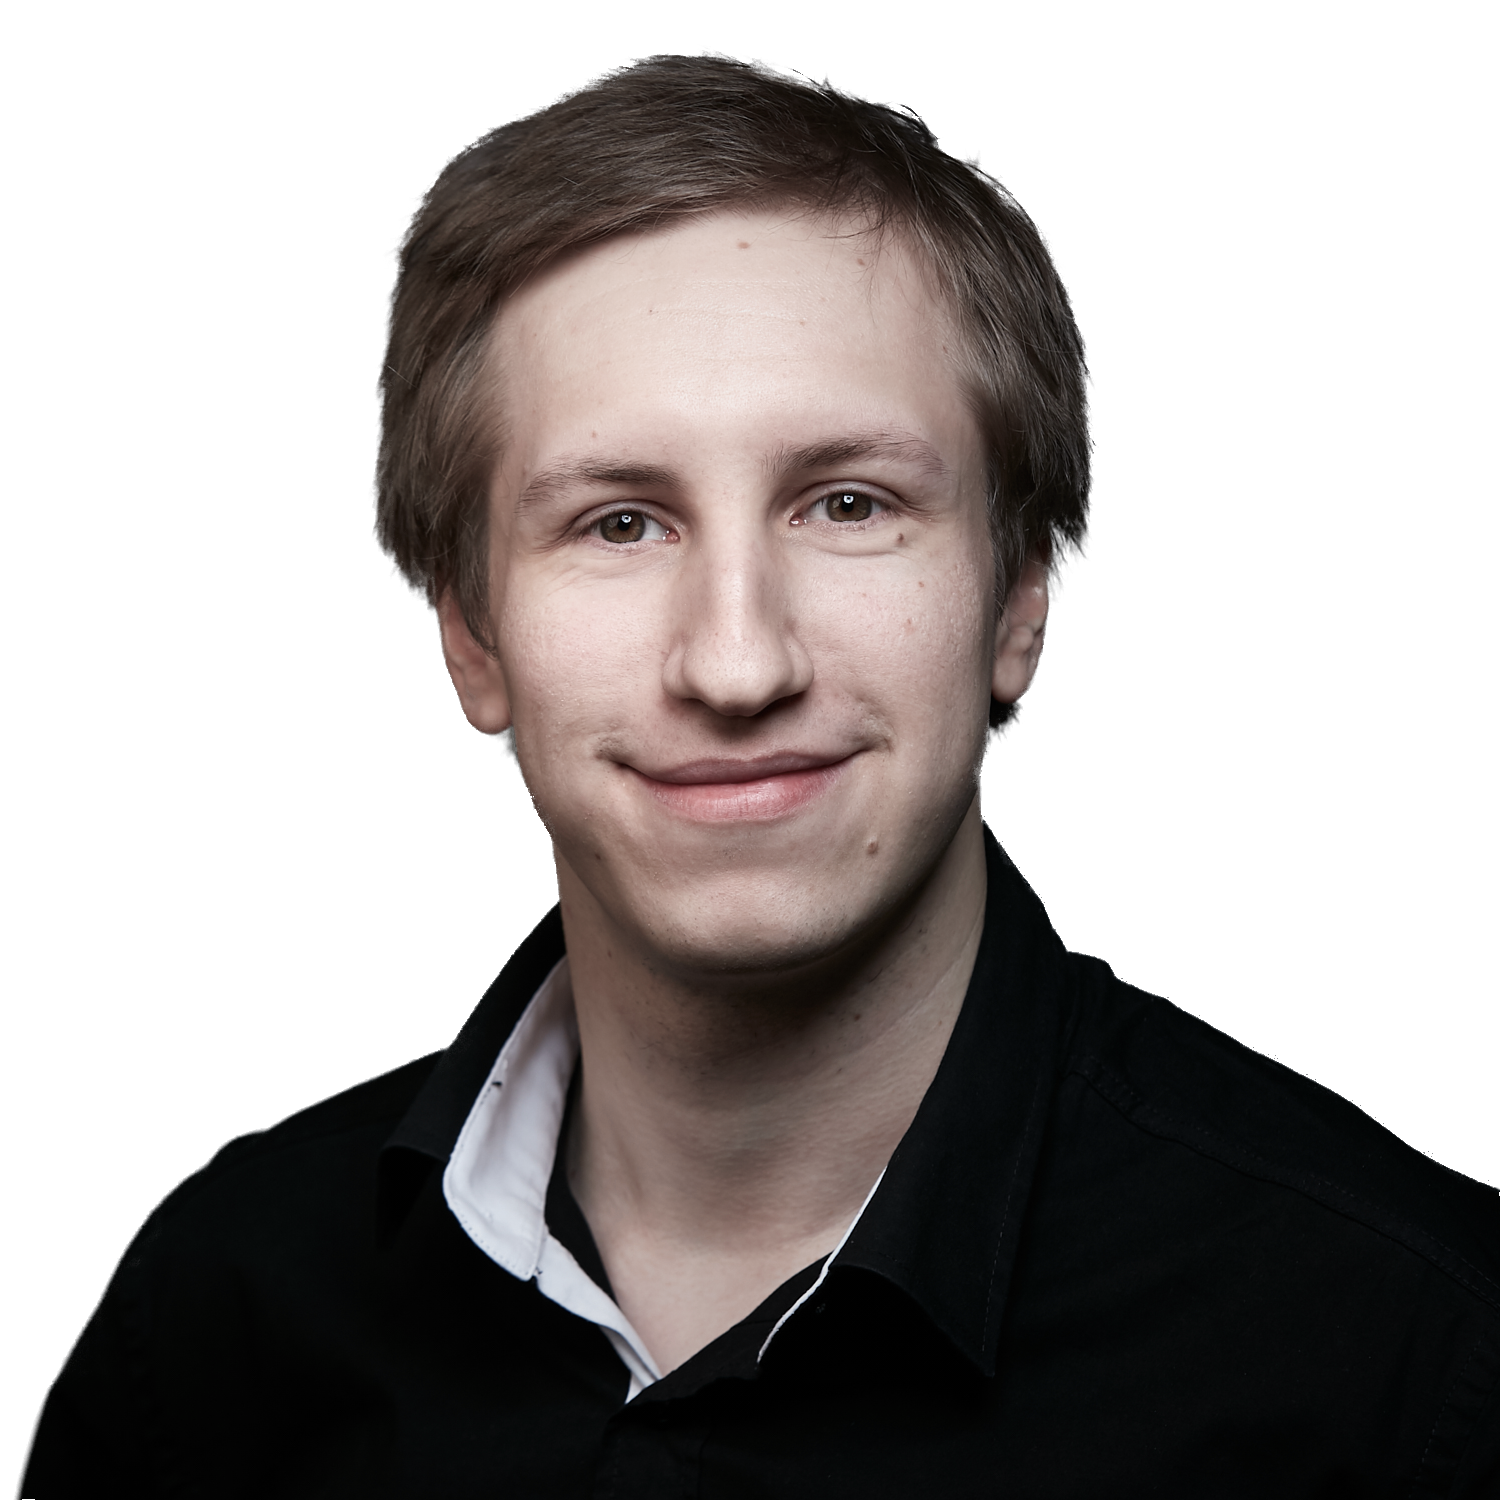
\includegraphics[width=\imagewidth]{max0.6.png}
				};
			\end{tikzpicture}
		\end{center}
		{\Large Max-Jonathan Luckow}
		{Computer Science Student\\}

		\begin{thyV}{2010}{2024}{21}{0.6\linewidth}
			\thyVent{high-school\\ diploma} 					{6/2010}
			\thyVent{Publication} 								{1/2020}
			\thyVent{B.Sc.\\Thesis} 							{3/2017}
			\thyVent{\\ M.Sc.Thesis} 							{3/2023}
			
			\thyVentEdu{Energy and\\Process Engineering} 		{4/2011}{9/2013} 	{}
			\thyVentEdu{Bachelor of Science \\Computer Science} {10/2013}{3/2017} 	{16.625/2014} 
			\thyVentEdu{Master of Science \\ Computer Science} 	{4/2017}{3/2023} 	{7.25/2020}

			\thyVentWork{Technical\\Accountant} 				{9/2020}{4/2022} 	{}
			\thyVentWork{Web Developer} 						{3/2018}{4/2018} 	{}
			\thyVentWork{Technical Specialist} 					{6/2017}{11/2017} 	{9.25/2017}
			\thyVentWork{Self-employed} 						{1/2014}{5/2017} 	{22.875/2014}

			\thyVentWork{Assistant in \\ surgical ward} 		{8/2010}{1/2011} 	{12.25/2010}
		\end{thyV}

		\thyLegend{Experience}{1.8cm}{thySecond} \thyLegend{Education}{1.8cm}{thyFirst} \thyLegend{Events}{1.1cm}{thyThird}
	\end{textblock}
	\begin{mdframed}
		\begin{minipage}[t]{0.50\textwidth}
			\vspace{-\baselineskip}
			\icon{Cross}{12}{30. Dezember 1990}\\
			\icon{Phone}{12}{+49 163 222 99 64}
		\end{minipage}
		\begin{minipage}[t]{0.50\textwidth} 
			\vspace{-\baselineskip}
			\icon{At}{12}{\href{mailto:max@luckow.ch}{max@luckow.ch}}\\
			\icon{Github}{12}{\href{https://github.com/Carlisle96}{github.com/Carlisle96}}
		\end{minipage}

		\thyVsection{Publication}{thyThird}
			M. J. Luckow and T. Fluschnik. \textbf{``\href{https://doi.org/10.1016/j.ipl.2019.105913}{On the Computational Complexity of Length- and Neighborhood-Constrained Path Problems}''}. In: \textit{Information Processing Letters.} Vol. 156 (2020). \hfill \textcolor{thyGrey}{1/2020}

		\begin{minipage}[t]{0.45\textwidth}
			\vspace{-\baselineskip}
			\thyVsection{Interests}{thyBlack}
			\vspace*{-12pt}
			\hspace{-12pt}\thyChart
		\end{minipage}
		\begin{minipage}[t]{0.55\textwidth} 
			\vspace{-\baselineskip}
			\thyVsection{Technical}{thyBlack}
				C/\Cplusplus, Java, Python \hfill \ThreeOfFour \\
				Latex \hfill \FourOfFour \\
				Haskell \hfill \OneOfFour \\
				Linux \hfill \ThreeOfFour \\
				Solidity \hfill \TwoOfFour \\
				%Javascript, Vue.js, Node.js, SQL \hfill \TwoOfFour \\
				Javascript \hfill \TwoOfFour \\
				Datev Uno \hfill \FourOfFour
		\end{minipage}
		\vspace*{-20pt}

		\thyVsection{Work Experience}{thySecond}
			\thyntry{Technical Acountant}{Agilo-Services GmbH}{9/2020 -- present}
			{Analysis, optimization and automation of the accounting system}
			{Datev Uno \slashsep Haskell}

			\thyntry{Web Developer}{Trado GmbH}{3/2018 -- 4/2018}
			{Implementation and maintenance of the internal administrative software}
			{Javascript \slashsep Node.js \slashsep Vue.js \slashsep SQL}

			\thyntryLast{Technical Specialist}{Envion AG}{6/2017 -- 11/2017}
					{Analysis of cryptocurrency market, devolopment of the first mining prototype and supervision of the production of the first large scale mining operation}
			    	{Linux \slashsep Solidity}

			%\thyntrySmall{Self-employed}{}{1/2014 -- 5/2017}
			%{IT administration, development and project support}

			%\thyntrySmall{Assistant in surgical ward}{Hospital Waldfriede Berlin}{08/2010 -- 01/2011}
			%{Community service}

		\thyVsection{Education}{thyFirst}

			\thyntry{Master of Science. Computer Science}{Technical University of Berlin}{4/2017 -- \textit{3/2013}}{Specialisation in cognitive systems}{Java \slashsep Python \slashsep Solidity}

			\thyntryLast{Bachelor of Science. Computer Science}{Technical University of Berlin}{4/2017 -- \textit{3/2013}}{Area of study in foundations of computing with the thesis on algorithms and complexity}{C/\Cplusplus \slashsep Java \slashsep Python \slashsep SQL \slashsep Latex}{}

			%\thyntrySmall{Energy and Process Engineering}{Technical University of Berlin}{4/2011 -- 9/2013}{}

			%\thyntrySmall{High-school diploma}{Arndt Gynasium Dahlem}{8/2003 -- 6/2010}{}

		\thyVsection{Language}{thyBlack}
			German: Native speaker \\
			English: Advanced \\
			Latin: Latinum


		\begin{textblock}{5}(17.5, 27.7)
			
\includegraphics[width=3cm]{signature2.png}
		\end{textblock}
	\end{mdframed}

\end{document}